\documentclass[tikz, border=10pt]{standalone}
\usepackage[T1]{fontenc}
\usepackage[utf8]{inputenc}
\usepackage{lmodern}
\usepackage[table]{xcolor}
\definecolor{IntelBlue}{HTML}{0068B5}
\definecolor{IntelLightBlue}{HTML}{DDEEF9}
\definecolor{FpgaOrange}{HTML}{E67E22}
\definecolor{FpgaLight}{HTML}{FDEBD0}
\definecolor{HpsGreen}{HTML}{1A7A4A}
\definecolor{HpsLight}{HTML}{D5F5E3}
\definecolor{GrayBg}{HTML}{F2F3F4}
\definecolor{GrayBorder}{HTML}{AAB7B8}
\definecolor{PassGreen}{HTML}{D5F5E3}
\definecolor{PassGreenDark}{HTML}{1E8449}
\definecolor{RowAlt}{HTML}{F7F9FB}
\definecolor{SummaryBg}{HTML}{EBF5FB}
\definecolor{NodeFill}{HTML}{D6EAF8}
\definecolor{NodeBorder}{HTML}{1B4F72}
\definecolor{InitFill}{HTML}{E5E7E9}
\definecolor{InitBorder}{HTML}{717D7E}
\definecolor{SleepFill}{HTML}{FEF5E7}
\definecolor{SleepBorder}{HTML}{935116}
\definecolor{MsgFill}{HTML}{D1F2EB}
\definecolor{MsgBorder}{HTML}{0E6655}
\definecolor{TimeoutRed}{HTML}{C0392B}
\definecolor{BtnBlue}{HTML}{1A5276}
\definecolor{ArrowGray}{HTML}{717D7E}
\usepackage{tikz}
\usetikzlibrary{shapes.geometric, arrows.meta, positioning, fit, backgrounds, calc, decorations.pathreplacing, bending, shadows.blur}
\begin{document}
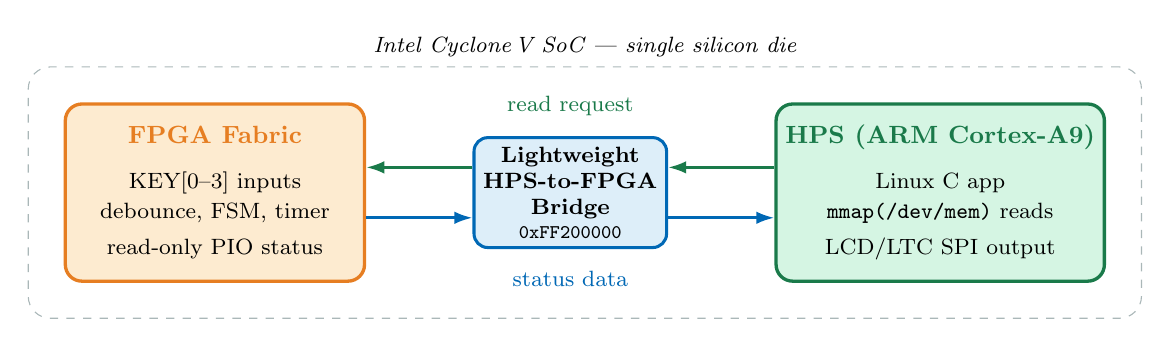
\begin{tikzpicture}[
  blk/.style={rectangle, rounded corners=6pt, minimum width=3.8cm,
              minimum height=2.25cm, align=center, font=\small,
              line width=1.2pt},
  bridge/.style={rectangle, rounded corners=5pt, minimum width=2.4cm,
                 minimum height=1.25cm, align=center,
                 font=\footnotesize\bfseries, draw=IntelBlue,
                 fill=IntelLightBlue, line width=1.1pt},
  lbl/.style={font=\footnotesize, fill=white, inner sep=2pt}
]
  \node[blk, draw=FpgaOrange, fill=FpgaLight] (fpga) {
    \textbf{\textcolor{FpgaOrange}{FPGA Fabric}}\\[5pt]
    \footnotesize KEY[0--3] inputs\\
    \footnotesize debounce, FSM, timer\\[2pt]
    \footnotesize read-only PIO status
  };
  \node[bridge, right=1.35cm of fpga] (bridge) {
    Lightweight\\HPS-to-FPGA\\Bridge\\[-1pt]
    \normalfont\scriptsize \texttt{0xFF200000}
  };
  \node[blk, draw=HpsGreen, fill=HpsLight, right=1.35cm of bridge] (hps) {
    \textbf{\textcolor{HpsGreen}{HPS (ARM Cortex-A9)}}\\[5pt]
    \footnotesize Linux C app\\
    \footnotesize \texttt{mmap(/dev/mem)} reads\\[2pt]
    \footnotesize LCD/LTC SPI output
  };
  \draw[-{Latex[length=2.3mm,width=1.6mm]}, line width=1.0pt,
        color=HpsGreen]
    ([yshift=0.32cm]hps.west) -- ([yshift=0.32cm]bridge.east);
  \draw[-{Latex[length=2.3mm,width=1.6mm]}, line width=1.0pt,
        color=HpsGreen]
    ([yshift=0.32cm]bridge.west) -- ([yshift=0.32cm]fpga.east);

  \draw[-{Latex[length=2.3mm,width=1.6mm]}, line width=1.0pt,
        color=IntelBlue]
    ([yshift=-0.32cm]fpga.east) -- ([yshift=-0.32cm]bridge.west);
  \draw[-{Latex[length=2.3mm,width=1.6mm]}, line width=1.0pt,
        color=IntelBlue]
    ([yshift=-0.32cm]bridge.east) -- ([yshift=-0.32cm]hps.west);

  \node[lbl, text=HpsGreen] at ($(bridge.north)+(0,0.38)$) {read request};
  \node[lbl, text=IntelBlue] at ($(bridge.south)+(0,-0.38)$) {status data};

  \node[draw=GrayBorder, dashed, rounded corners=8pt,
        fit=(fpga)(bridge)(hps), inner sep=0.45cm,
        label={[font=\footnotesize\itshape]above:Intel Cyclone\,V SoC --- single silicon die}] {};
\end{tikzpicture}
\end{document}
